\documentclass[12pt,a4paper]{article}

% --- PACKAGES ---
\usepackage[utf8]{inputenc}
\usepackage[T1]{fontenc}        % Font encoding
\usepackage{amsmath}
\usepackage{amsfonts}           % Math fonts package
\usepackage{amssymb}            % Math symbols package
\usepackage{graphicx}           % Required for including images
\usepackage[a4paper, margin=1in]{geometry} % For page margins
\usepackage{times}              % Uses Times New Roman like font
\usepackage{setspace}           % For line spacing
\usepackage{hyperref}           % For clickable links

\usepackage{fancyhdr}           % For custom headers and footers
\usepackage{caption}            % For customizing captions
% \usepackage{subcaption}       % For subfigures (if needed)
% \usepackage{float}            % For better figure placement with [H] (if needed)
% \usepackage{tikz}             % For diagrams (if needed)
% \usetikzlibrary{shapes.geometric, arrows, positioning, fit} % TikZ libraries (if needed)

\usepackage{xcolor}
\usepackage{sectsty}            % To style section headings
\usepackage{tocloft}            % To style Table of Contents
\usepackage{listings}           % For code listings

% --- COLOR DEFINITIONS ---
\definecolor{RoyalBlue}{RGB}{0, 0, 128} % As per your example
\definecolor{codegreen}{rgb}{0,0.6,0}
\definecolor{codegray}{rgb}{0.5,0.5,0.5}
\definecolor{codepurple}{rgb}{0.58,0,0.82}
\definecolor{backcolour}{rgb}{0.95,0.95,0.92}

% --- HYPERREF SETUP ---
\hypersetup{
    colorlinks=true,
    linkcolor=RoyalBlue,
    filecolor=magenta,      
    urlcolor=cyan, % Kept cyan for URLs, you can change to RoyalBlue if preferred
    pdftitle={Understanding Structural Design Patterns: Flyweight and Facade}, % Corrected PDF title
    pdfpagemode=FullScreen,
}

% --- FONT & SECTION STYLING ---
\sectionfont{\color{RoyalBlue}}    % Section titles in document
\subsectionfont{\color{RoyalBlue}} % Subsection titles
\subsubsectionfont{\color{RoyalBlue}}% Subsubsection titles

% --- TABLE OF CONTENTS STYLING ---
\renewcommand{\cfttoctitlefont}{\color{black}\Huge\bfseries} % Title "Contents" in black
\renewcommand{\cftsecfont}{\color{RoyalBlue}}              % Section entries in ToC
\renewcommand{\cftsecpagefont}{\color{RoyalBlue}}          % Section page numbers
\renewcommand{\cftsubsecfont}{\color{RoyalBlue}}           % Subsection entries
\renewcommand{\cftsubsecpagefont}{\color{RoyalBlue}}       % Subsection page numbers
\renewcommand{\cftsubsubsecfont}{\color{RoyalBlue}}        % Subsubsection entries
\renewcommand{\cftsubsubsecpagefont}{\color{RoyalBlue}}    % Subsubsection page numbers

% --- LISTINGS (CODE) SETUP ---
\lstdefinestyle{mystyle}{
    backgroundcolor=\color{backcolour},   
    commentstyle=\color{codegreen},
    keywordstyle=\color{magenta},
    numberstyle=\tiny\color{codegray},
    stringstyle=\color{codepurple},
    basicstyle=\ttfamily\footnotesize,
    breakatwhitespace=false,          
    breaklines=true,                  
    captionpos=b,                     
    keepspaces=true,                  
    numbers=left,                     
    numbersep=5pt,                    
    showspaces=false,                 
    showstringspaces=false,
    showtabs=false,                   
    tabsize=2,
    frame=single,
    rulecolor=\color{black}, % Frame color for listings
    title=\lstname % To show the filename if provided in caption
}
\lstset{style=mystyle}

% --- PAGE STYLE FOR CONTENT PAGES ---
\pagestyle{fancy}
\fancyhf{} % Clear all header and footer fields
\fancyhead[C]{\textit{Structural Design Patterns: Flyweight and Facade}} % Corrected Custom header
\fancyfoot[C]{\thepage}
\renewcommand{\headrulewidth}{0.4pt}
\renewcommand{\footrulewidth}{0pt} % No footer rule

% --- CUSTOM TITLE PAGE COMMAND ---
\newcommand{\maketitlepage}{
    \begin{titlepage}
        \centering
        \vspace*{0.5cm}
        % 
\includegraphics[width=0.25\textwidth]{RUET_logo.png} % Placeholder for University Logo
        {\Huge \textbf{RAJSHAHI UNIVERSITY OF ENGINEERING \& TECHNOLOGY}}
        \vspace*{0.5cm}
        {\Large Department of Computer Science and Engineering}
        
        \vspace*{2.5cm}
        
        {\huge\bfseries Understanding Structural Design Patterns: \\ Flyweight and Facade\par} % Reverted to original title
        \vspace{0.5cm}
        {\Large \textit{A Software Engineering Sessional Project Report}\par} % Subtitle
        
        \vspace{2cm}
        
        \begin{flushleft}
        \large \textbf{Submitted by:}\\
        \large Md Naim Parvez \\ % Keep user's specific name/roll if they prefer, or indicate placeholder
        \large Roll No: 2003015 \\
        \large Section: A \\
        \large Third Year (Even Semester) \\ % Assuming, adjust if needed
        \end{flushleft}
        
        \vspace{1cm}
        
        \begin{flushleft}
        \large \textbf{Submitted to:}\\
        \large Emrana Kabir Hashi \\
        \large Assistant Professor \\
        \large Department of Computer Science and Engineering \\
        \large Rajshahi University of Engineering \& Technology (RUET) \\
        \end{flushleft}
        
        \vspace{1cm}
        {\large \textbf{Course Code:} CSE 3206} \\
        {\large \textbf{Course Title:} Software Engineering Sessional}
        
        \vfill 
        
        {\large April 2025\par} % Submission Date (Matches previous content)
    \end{titlepage}
}

% --- BEGIN DOCUMENT ---
\begin{document}

\maketitlepage % Calls the command to generate the title page

\clearpage % Ensures the Table of Contents starts on a new page
\tableofcontents % Generates the Table of Contents
\clearpage % Ensures the main content starts on a new page after the TOC

% --- REPORT CONTENT STARTS HERE ---

\section{Introduction to Design Patterns}
Design patterns provide a proven approach to solving recurring challenges in software design. They serve as a common vocabulary for developers, enabling more efficient communication and collaboration. These patterns are not ready-made code snippets that can be directly transformed into code; rather, they are guidelines for solving particular problems in software design. Design patterns are typically categorized into three main types: Creational Patterns (focus on object creation mechanisms), Structural Patterns (focus on object composition and relationships), and Behavioral Patterns (focus on communication between objects). This report will specifically explore two significant structural design patterns: Flyweight and Facade, examining how they contribute to optimizing resource utilization and simplifying complex system interfaces, respectively.

\section{The Flyweight Design Pattern}

\subsection{Overview}
The Flyweight pattern is a structural design pattern that aims to minimize memory usage by sharing as much data as possible with similar objects. It is particularly useful when an application needs to create a large number of similar objects that would otherwise consume excessive memory.

\subsection{Key Concepts}
The Flyweight pattern distinguishes between two types of state:
\begin{itemize}
    \item \textbf{Intrinsic State (Shared Data):} This consists of information that can be shared across multiple objects because it doesn't change and is context-independent. This data is stored in the flyweight object.
    \item \textbf{Extrinsic State (Unique Data):} This is context-dependent information that cannot be shared and must be passed to the flyweight when its operations are invoked.
\end{itemize}
The major components of the Flyweight pattern include:
\begin{itemize}
    \item \textbf{Flyweight:} An interface or abstract class defining the operations that can accept extrinsic state.
    \item \textbf{Concrete Flyweight:} Implements the Flyweight interface and stores intrinsic state.
    \item \textbf{Flyweight Factory:} Creates and manages flyweight objects, ensuring they are shared properly.
    \item \textbf{Client:} Maintains references to flyweights and computes or stores the extrinsic state.
\end{itemize}

\subsection{Real-World Analogy}
A classic real-world analogy for the Flyweight pattern is a chess game: Instead of creating separate objects for each chess piece on the board (which would consume a lot of memory), one can create only one object for each type of piece (King, Queen, Pawn, etc.) storing their appearance and behavior (intrinsic state). The position of each piece is stored separately as extrinsic state. This way, a game with 32 pieces on the board would only need 6 unique piece objects, with their positions on the board managed separately.

\subsection{Case Study: Tree Rendering in a Forest Simulation}
Consider a graphics application or a game that needs to render a vast forest with thousands of trees. Each tree might have common properties like its species (oak, pine), texture, and general mesh structure. However, each tree also has unique properties like its precise coordinates, height, and health. Using the Flyweight pattern, we can share the common "tree type" data while keeping individual tree instances very lightweight.

\subsubsection{Problem Statement}
Efficiently rendering a large number of unique tree instances in a forest simulation poses challenges related to:
\begin{itemize}
    \item High memory consumption due to duplicated graphical and structural data for each tree.
    \item Performance bottlenecks when drawing or updating individual tree objects if their full data is stored separately.
    \item Maintaining a clear separation between shared, static tree properties and their dynamic, unique positions and states.
\end{itemize}

\subsubsection{Implementation in Python}
\begin{lstlisting}[language=Python, caption={Python Implementation for Flyweight Pattern (Tree Rendering)}, label={lst:flyweight_tree_rendering}]
# tree_rendering_flyweight.py

# Intrinsic State (shared among many trees of the same type)
class TreeType:
    def __init__(self, name, color, texture):
        self.name = name
        self.color = color
        self.texture = texture
        print(f"Creating new TreeType (Flyweight): {name}, {color}, {texture}")

    def draw(self, canvas, x, y, height, health_status):
        # This method uses both intrinsic (self.name, etc.)
        # and extrinsic (x, y, height, health_status) data.
        # In a real app, 'canvas' would be a graphics context.
        print(f"Drawing {self.color} {self.name} at ({x},{y}) with height {height}m and health {health_status}. Texture: {self.texture}")

# Flyweight Factory
class TreeFactory:
    _tree_types = {}

    def get_tree_type(self, name, color, texture):
        key = (name, color, texture)
        if key not in self._tree_types:
            self._tree_types[key] = TreeType(name, color, texture)
        return self._tree_types[key]

# Contextual Object (holds extrinsic state and references the flyweight)
class Tree:
    def __init__(self, x, y, tree_type_flyweight, height, health_status):
        self.x = x
        self.y = y
        self.tree_type = tree_type_flyweight # Reference to shared flyweight
        self.height = height # Extrinsic
        self.health_status = health_status # Extrinsic

    def render(self, canvas):
        self.tree_type.draw(canvas, self.x, self.y, self.height, self.health_status)

# Client (Forest simulation)
class Forest:
    def __init__(self):
        self.trees = []
        self.factory = TreeFactory()

    def plant_tree(self, x, y, name, color, texture, height, health_status):
        tree_type = self.factory.get_tree_type(name, color, texture)
        tree = Tree(x, y, tree_type, height, health_status)
        self.trees.append(tree)

    def draw(self, canvas):
        print("\n--- Rendering Forest ---")
        for tree in self.trees:
            tree.render(canvas)

# Main simulation loop
if __name__ == "__main__":
    forest_sim = Forest()

    # Planting many trees, reusing TreeType objects
    forest_sim.plant_tree(10, 10, "Oak", "Green", "oak_bark.png", 20, "Healthy")
    forest_sim.plant_tree(12, 15, "Pine", "Dark Green", "pine_needles.png", 30, "Healthy")
    forest_sim.plant_tree(11, 12, "Oak", "Green", "oak_bark.png", 18, "Diseased")
    forest_sim.plant_tree(20, 25, "Oak", "Green", "oak_bark.png", 22, "Healthy")
    forest_sim.plant_tree(5, 8, "Pine", "Dark Green", "pine_needles.png", 28, "Healthy")

    forest_sim.draw("MainCanvas") # 'MainCanvas' is a placeholder for a graphics context
\end{lstlisting}

\subsubsection{Output}
When executed, the program produces the following output, demonstrating how `TreeType` (Flyweight) objects are created once per unique type and then reused:
\begin{verbatim}
Creating new TreeType (Flyweight): Oak, Green, oak_bark.png
Creating new TreeType (Flyweight): Pine, Dark Green, pine_needles.png

--- Rendering Forest ---
Drawing Green Oak at (10,10) with height 20m and health Healthy. Texture: oak_bark.png
Drawing Dark Green Pine at (12,15) with height 30m and health Healthy. Texture: pine_needles.png
Drawing Green Oak at (11,12) with height 18m and health Diseased. Texture: oak_bark.png
Drawing Green Oak at (20,25) with height 22m and health Healthy. Texture: oak_bark.png
Drawing Dark Green Pine at (5,8) with height 28m and health Healthy. Texture: pine_needles.png
\end{verbatim}
\begin{figure}[htbp]
    \centering
    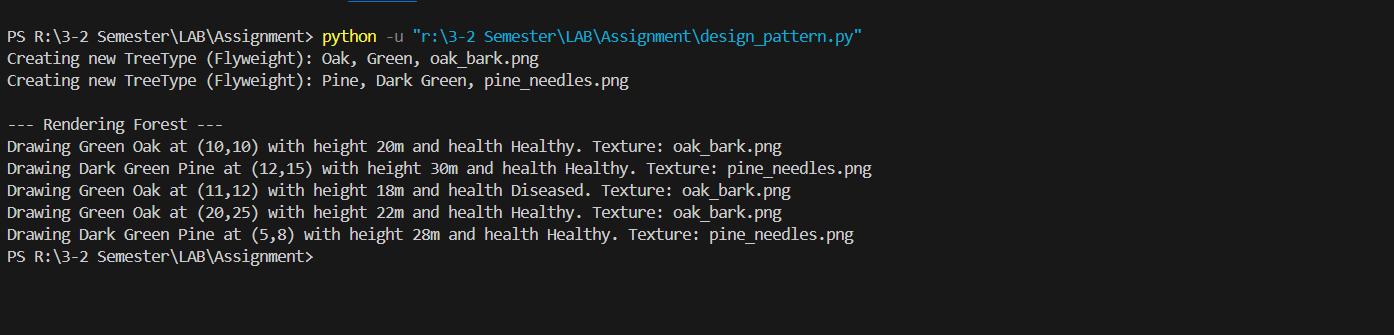
\includegraphics[width=0.7\textwidth]{flyweight.png}
    \caption{Output of the Flyweight Pattern: Tree Rendering in a Forest Simulation}
    \label{fig:flyweight_uml}
\end{figure}
This output clearly shows that `TreeType` objects (flyweights) are created only once for each unique combination of `name`, `color`, and `texture`, even though multiple `Tree` instances reference them. This demonstrates the memory optimization achieved by sharing the intrinsic state for graphical assets and common properties.


\subsection{Benefits and Limitations}
\subsubsection{Benefits}
\begin{itemize}
    \item Significant memory savings when dealing with a large number of similar objects.
    \item Improved performance due to reduced memory consumption.
    \item Centralized management of shared state.
\end{itemize}

\subsubsection{Limitations}
\begin{itemize}
    \item Increased complexity in code structure.
    \item Potential runtime cost of transferring extrinsic state.
    \item Works best when shared state is immutable.
\end{itemize}

\section{The Facade Design Pattern}

\subsection{Overview}
The Facade design pattern is another structural pattern that provides a simplified interface to a complex subsystem of classes. It acts as a "front-facing" interface that masks more complex underlying or structural code. The primary goal is to reduce complexity for the client and minimize dependencies on the subsystem.

\subsection{Key Concepts}
The Facade pattern consists of the following components:
\begin{itemize}
    \item \textbf{Facade:} Provides a simplified interface to a set of interfaces in a subsystem.
    \item \textbf{Subsystem Classes:} Complex classes that implement the functionality of the subsystem.
    \item \textbf{Client:} Interacts with the subsystem through the Facade.
\end{itemize}
The Facade doesn't encapsulate the subsystem classes; it just provides a simplified interface to their functionality. Clients can still access the subsystem classes directly if needed.

\subsection{Real-World Analogy}
A real-world analogy for the Facade pattern is a home theater system: When you want to watch a movie, you need to turn on the TV, set up the sound system, turn on the DVD or streaming device, dim the lights, and start the movie. Instead of performing each step individually, a home theater facade (like a universal remote with a "Movie Mode" button) can simplify this process, hiding the complexity of the individual components and providing a single, simplified interface to the user.

\subsection{Case Study: Complex Report Generation System}
Consider a system designed to generate various types of reports (e.g., financial, sales, inventory). This process involves multiple complex backend subsystems: a Data Fetcher, a Data Processor, a Report Formatter, and a Notification Service. Without a facade, a client application would need to interact with each of these components directly, managing their dependencies and orchestration.

\subsubsection{Problem Statement}
Generating comprehensive reports from diverse data sources presents several challenges:
\begin{itemize}
    \item High coupling between the client application and multiple intricate backend data processing and formatting modules.
    \item Duplication of complex orchestration logic across different client sections or report types.
    \item Difficulty for new developers to quickly grasp the end-to-end process of generating a report.
\end{itemize}

\subsubsection{Implementation in Python}
\begin{lstlisting}[language=Python, caption={Python Implementation for Facade Pattern (Report Generation System)}, label={lst:facade_report_generation}]
import time
import datetime

# Subsystem 1: Data Fetcher
class DataFetcher:
    def fetch_sales_data(self, start_date, end_date):
        print(f"DataFetcher: Fetching sales data from {start_date} to {end_date}...")
        time.sleep(0.5) # Simulate network delay
        return [{"product": "Laptop", "sales": 100}, {"product": "Mouse", "sales": 250}]

    def fetch_inventory_data(self):
        print("DataFetcher: Fetching inventory data...")
        time.sleep(0.3)
        return [{"item": "Laptop", "stock": 50}, {"item": "Keyboard", "stock": 150}]

# Subsystem 2: Data Processor
class DataProcessor:
    def aggregate_sales(self, raw_data):
        print("DataProcessor: Aggregating sales data...")
        total_sales = sum(item["sales"] for item in raw_data)
        return {"total_sales": total_sales, "items": raw_data}

    def calculate_stock_value(self, inventory_data, prices):
        print("DataProcessor: Calculating inventory value...")
        total_value = sum(item["stock"] * prices.get(item["item"], 0) for item in inventory_data)
        return {"total_stock_value": total_value, "items": inventory_data}

# Subsystem 3: Report Formatter
class ReportFormatter:
    def format_sales_report(self, processed_data):
        print("ReportFormatter: Formatting sales report...")
        report_str = f"Sales Report ({datetime.date.today()}):\n"
        report_str += f"Total Sales: ${processed_data['total_sales']}\n"
        for item in processed_data['items']:
            report_str += f"  - {item['product']}: {item['sales']} units\n"
        return report_str

    def format_inventory_report(self, processed_data):
        print("ReportFormatter: Formatting inventory report...")
        report_str = f"Inventory Report ({datetime.date.today()}):\n"
        report_str += f"Total Inventory Value: ${processed_data['total_stock_value']:.2f}\n"
        for item in processed_data['items']:
            report_str += f"  - {item['item']}: {item['stock']} units\n"
        return report_str

# Subsystem 4: Notification Service
class NotificationService:
    def send_email(self, recipient, subject, body):
        print(f"NotificationService: Sending email to {recipient} with subject '{subject}'")
        # In a real app, this would integrate with an email API
        print(f"Email Body:\n---\n{body}\n---")
        time.sleep(0.1)

# Facade Class
class ReportGenerationFacade:
    def __init__(self):
        self.data_fetcher = DataFetcher()
        self.data_processor = DataProcessor()
        self.report_formatter = ReportFormatter()
        self.notification_service = NotificationService()
        self.product_prices = {"Laptop": 1200, "Mouse": 25, "Keyboard": 75} # Sample prices

    def generate_and_send_daily_sales_report(self, recipient_email):
        print("\n--- Initiating Daily Sales Report Generation ---")
        today = datetime.date.today()
        yesterday = today - datetime.timedelta(days=1)
        
        # 1. Fetch data
        raw_sales = self.data_fetcher.fetch_sales_data(yesterday, today)
        
        # 2. Process data
        processed_sales = self.data_processor.aggregate_sales(raw_sales)
        
        # 3. Format report
        sales_report_content = self.report_formatter.format_sales_report(processed_sales)
        
        # 4. Send notification
        self.notification_service.send_email(
            recipient_email,
            f"Daily Sales Report - {today}",
            sales_report_content
        )
        print("--- Daily Sales Report Process Completed ---")

    def generate_and_check_inventory_value(self):
        print("\n--- Initiating Inventory Value Check ---")
        # 1. Fetch data
        inventory_data = self.data_fetcher.fetch_inventory_data()
        
        # 2. Process data
        calculated_value = self.data_processor.calculate_stock_value(inventory_data, self.product_prices)
        
        # 3. Format report (optional, can just return value)
        inventory_report_content = self.report_formatter.format_inventory_report(calculated_value)

        print(inventory_report_content)
        print(f"Current Total Inventory Value: ${calculated_value['total_stock_value']:.2f}")
        print("--- Inventory Value Check Completed ---")
        return calculated_value['total_stock_value']

# Client Code
if __name__ == "__main__":
    report_system = ReportGenerationFacade()

    # Client uses the facade to perform a complex task simply
    report_system.generate_and_send_daily_sales_report("manager@example.com")

    # Another complex task via the facade
    current_inventory_value = report_system.generate_and_check_inventory_value()
    print(f"\nFinal Check: Inventory value reported as ${current_inventory_value:.2f}")

\end{lstlisting}

\subsubsection{Output}
When executed, the system produces the following log output:
\begin{verbatim}
--- Initiating Daily Sales Report Generation ---
DataFetcher: Fetching sales data from 2025-04-14 to 2025-04-15...
DataProcessor: Aggregating sales data...
ReportFormatter: Formatting sales report...
NotificationService: Sending email to manager@example.com with subject 'Daily Sales Report - 2025-04-15'
Email Body:
---
Sales Report (2025-04-15):
Total Sales: $350
  - Laptop: 100 units
  - Mouse: 250 units
---
--- Daily Sales Report Process Completed ---

--- Initiating Inventory Value Check ---
DataFetcher: Fetching inventory data...
DataProcessor: Calculating inventory value...
ReportFormatter: Formatting inventory report...
Inventory Report (2025-04-15):
Total Inventory Value: $7250.00
  - Laptop: 50 units
  - Keyboard: 150 units
Current Total Inventory Value: $7250.00
--- Inventory Value Check Completed ---

Final Check: Inventory value reported as $7250.00
\end{verbatim}
\begin{figure}[htbp]
    \centering
    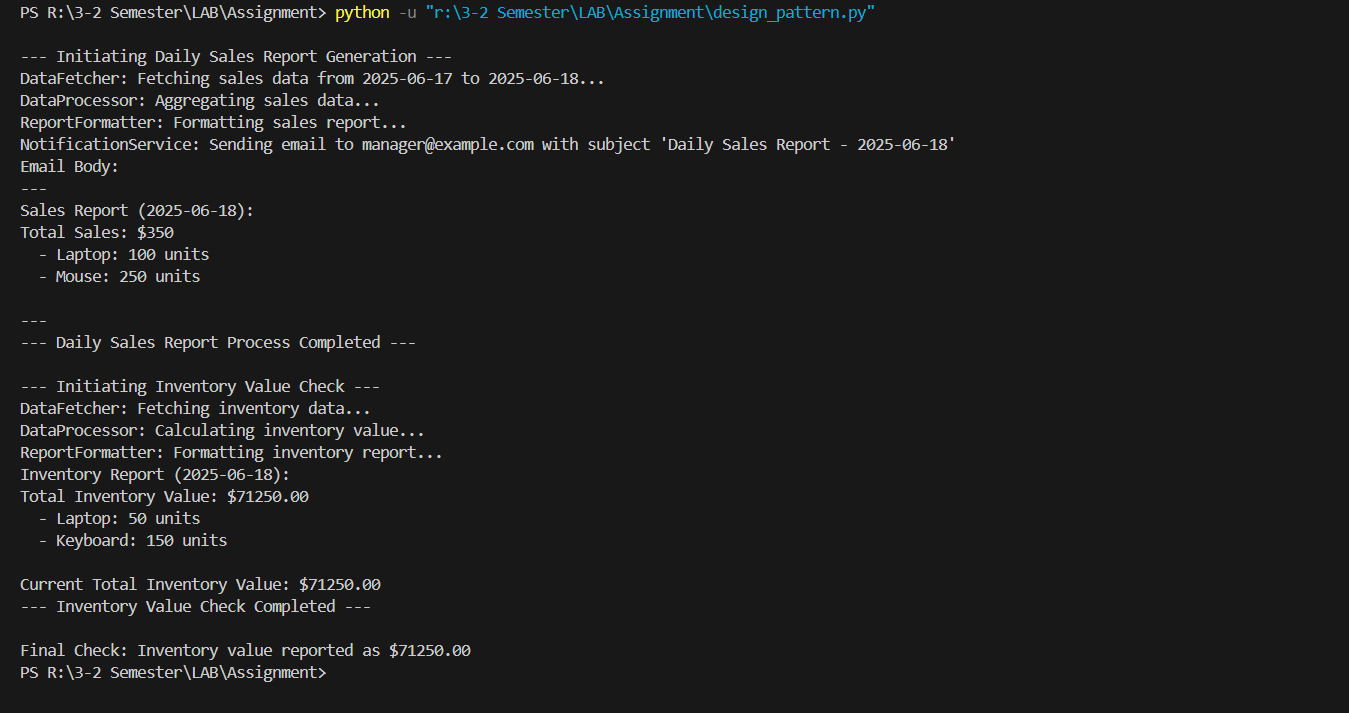
\includegraphics[width=0.7\textwidth]{facade.png}
    \caption{Output of the Facade Pattern: Simplified Report Generation Process}
    \label{fig:facade_uml}
\end{figure}

This demonstrates how the `ReportGenerationFacade` orchestrates calls to multiple underlying subsystem classes (DataFetcher, DataProcessor, ReportFormatter, NotificationService) through simple, high-level methods. The client only needs to interact with the facade, significantly simplifying its code and reducing its dependency on the individual complex components.

\subsection{Benefits and Limitations}
\subsubsection{Benefits}
\begin{itemize}
    \item Simplifies client interaction with complex subsystems.
    \item Promotes loose coupling between client and subsystem.
    \item Enhances code readability and maintainability.
    \item Facilitates easier testing and debugging.
\end{itemize}

\subsubsection{Limitations}
\begin{itemize}
    \item May hide too much complexity, limiting access to advanced features.
    \item Can create an overdependence on the facade.
    \item Requires regular maintenance to stay in sync with subsystem changes.
\end{itemize}

\section{Comparing Flyweight and Facade Patterns}
While both Flyweight and Facade are structural design patterns, they serve different purposes and solve different problems.

\begin{itemize}
    \item \textbf{Purpose:}
    \begin{itemize}
        \item \textbf{Flyweight:} Focuses on memory optimization by sharing common data.
        \item \textbf{Facade:} Focuses on simplifying interfaces to complex subsystems.
    \end{itemize}
    \item \textbf{Problem Solved:}
    \begin{itemize}
        \item \textbf{Flyweight:} Solves the problem of high memory consumption with many similar objects.
        \item \textbf{Facade:} Solves the problem of complex interactions with subsystems.
    \end{itemize}
    \item \textbf{Implementation Strategy:}
    \begin{itemize}
        \item \textbf{Flyweight:} Divides object state into shared and unique parts.
        \item \textbf{Facade:} Provides a unified interface to a set of interfaces in a subsystem.
    \end{itemize}
    \item \textbf{Client Interaction:}
    \begin{itemize}
        \item \textbf{Flyweight:} In Flyweight, clients need to manage the extrinsic state.
        \item \textbf{Facade:} In Facade, clients interact with a simpler interface that handles complexity behind the scenes.
    \end{itemize}
\end{itemize}

\section{Conclusion}
The Flyweight and Facade design patterns represent two different approaches to managing complexity in software systems. The Flyweight pattern optimizes memory usage by sharing common data among multiple similar objects, making it ideal for scenarios involving large numbers of similar objects. The Facade pattern simplifies complex subsystems by providing a unified interface, making it easier for clients to interact with these systems without understanding their internal workings. Both patterns demonstrate the importance of structural design in software engineering. When applied correctly, they can significantly improve software quality by enhancing memory efficiency, reducing complexity, and promoting loose coupling between components. By understanding and applying these design patterns, software developers can create more efficient, maintainable, and scalable applications that better meet the needs of users and businesses.

\end{document}
